% !TeX root = ../main.tex

\chapter{编译器后端设计实现}



\section{去糖化}

语法糖是由英国计算机科学家彼得·兰丁发明的一个术语,
指计算机语言中添加的某种语法,这种语法对语言的功能没有影响,
但是更方便程序员使用。
语法糖让程序更加简洁,有更高的可读性。

一个实用的通用编程语言会提供非常多的功能,但从语言实现的角度考虑,
在编译之前将语言的某些部分转换成使用其他更核心的部分来实现,
能让语言维持一个比较小的核心,以便更容易维护同时也更具灵活性。
我们把该步骤称为去糖化,对应的编译过程(pass)称为 shrink。

本文实现的语言中,布尔与、或运算并不属于核心语言,它们会被编译成 if 语句。
\begin{small}
\begin{align*}
  \CAND{e_1}{e_2} & \quad \Rightarrow \quad \CIF{e_1}{e_2}{\FALSE{}}\\
  \COR{e_1}{e_2} & \quad \Rightarrow \quad \CIF{e_1}{\TRUE{}}{e_2}
\end{align*}
\end{small}

这个转换维持了与、或运算的短路特性。该转换的代码实现如下:

\begin{lstlisting}
(define (shrink-exp e)
  (match e
    [(or (Int _) (Var _) (Bool _) (Void))
     e]
    [(Let x rhs body)
     (Let x (shrink-exp rhs) (shrink-exp body))]
    [(Prim 'and (list e1 e2))
     (If (shrink-exp e1)
         (shrink-exp e2)
         (Bool #f))]
    [(Prim 'or (list e1 e2))
     (If (shrink-exp e1)
         (Bool #t)
         (shrink-exp e2))]
    [(Prim op es) (Prim op (map shrink-exp es))]
    ...
\end{lstlisting}

代码中出现的\code{\#t, \#f}与\code{true, false}相同。
这里处理程序,或者说操作语法树的方法是使用自然递归,也叫结构化递归,
即在结构的子结构上进行递归。
例如,在转换与、或运算时,先对两个运算数进行递归转换,
然后把转换的结果放入 if 表达式中。
这样我们就可以处理任意复杂的与、或运算。
后面的绝大部分编译过程也是如此。


% !TeX root = ../../main.tex

\section{标识符唯一化}

由于 x86-64 以及后面使用的线性的中间代码不具备作用域,
也为了方便后续对程序进行分析,
我们需要确保所有的标识符的名字是唯一的,包括变量名和参数名,
就像下面这样。

以 let 语句为例,标识符唯一化将进行如下的转换:
\begin{transformation}
\begin{lstlisting}
(let ([x (let ([x 4])
            (+ x 1))])
  (+ x 2))
\end{lstlisting}
\compilesto
\begin{lstlisting}
(let ([x2 (let ([x1 4])
              (+ x1 1))])
  (+ x2 2))
\end{lstlisting}
\end{transformation}

这个编译过程的实现如下:

\begin{lstlisting}
(define ((uniquify-exp env) e)
  (define recur (uniquify-exp env))
  (match e
    [(or (Int _) (Bool _) (Void)) e]
    [(Var x) (Var (dict-ref env x))]
    [(Let x e body)
     (let ([new-x (gensym x)])
       (Let new-x
            (recur e)
            ((uniquify-exp (dict-set env x new-x)) body)))]
    [(If e1 e2 e3)
     (If (recur e1) (recur e2) (recur e3))]
    [(SetBang x e)
     (SetBang (dict-ref env x) (recur e))]
    ...
\end{lstlisting}

这时处理语法树的递归函数上除了当前结点这一参数外,
还多了一个 env 参数,这个参数是一个字典,
每当绑定一个变量时,
我们使用 \code{gensym} 函数生成一个全局唯一的符号作为新变量名,
并在字典中加入新的键值对,键为变量名,值为新变量名。
使用变量时,也就是访问变量或对变量赋值时,
我们查找这个字典,对变量名进行替换。
函数的参数也需要进行相同的处理。
在遇到函数定义时把原参数名和新生成的唯一参数名作为键值对加入字典,
在函数体内使用该字典进行标识符替换。

其中,\code{gensym} 可以接受一个字符串或符号参数,
生成的符号将以这个参数作为前缀。
例如\code{(gensym 'print)}将会生成类似\code{print46352}的符号。
这个功能可以帮助我们生成更易读、易调试的中间代码。


% !TeX root = ../../main.tex

\section{赋值转换}

考虑这样的例子:

\begin{multilinecode}
\begin{lstlisting}
(let ([x 2])
  (+ x
     (begin (set! x 40) x)))
\end{lstlisting}
\end{multilinecode}

其中 begin 语句接受若干个表达式,依次执行,然后将最后一个表达式的结果返回。
由于在我们的语言中,操作数先依次从左往右被求值,然后执行运算,
上面的代码应该得到 42。

因为汇编语言的运算符的操作数不支持复杂表达式,
而仅仅支持立即数或者从一个寄存器或内存地址中获取操作数。
在后面有一趟被称作原子化操作数的编译过程,会把所有复杂的操作数提取出来,
求值后赋值给一个临时变量,用这个临时变量替换原来的复杂操作数。
像下面这样:

\begin{transformation}
\begin{lstlisting}
      (+ (+ x 1) 2)
\end{lstlisting}
\compilesto
\begin{lstlisting}
    (let ([tmp (+ x 1)])
      (+ tmp 2))
\end{lstlisting}
\end{transformation}

但是对于上面包含赋值的例子,如果我们只是进行简单的提取替换,会得到下面的结果:

\begin{multilinecode}
\begin{lstlisting}
(let ([x 2])
  (let ([tmp (begin (set! x 40) x)])
    (+ x tmp)))
\end{lstlisting}
\end{multilinecode}

由于对 x 重新赋值的语句原来处于操作数的位置,它会被提取到加法运算的前面。
显然,转换后的程序会得到错误的结果:80。

解决的方法是对于所有涉及到被重新赋值的变量,
我们把对它们的读取包裹在一个复杂操作 get 的后面。
当然,在最终翻译成汇编代码时,通过 get 语句访问变量和直接访问变量并没有区别。
上面的程序将被转换成这样:

\begin{multilinecode}
\begin{lstlisting}
(let ([x 2])
  (+ (get! x)
     (begin (set! x 40)
            (get! x))))
\end{lstlisting}
\end{multilinecode}

这样一来,对这些变量的读取也会被提取到运算之前。
只要原子化操作数这一过程按正确的顺序提取复杂操作数,
我们就能得到正确的程序:

\begin{multilinecode}
\begin{lstlisting}
(let ([x 2])
  (let ([tmp1 (get! x)])
    (let ([tmp2 (begin (set! x 40)
                       (get! x))])
      (+ tmp1 tmp2))))
\end{lstlisting}
\end{multilinecode}

赋值还会导致在编译闭包时出现另一个问题,
我们将在后文描述闭包的实现时指出。


% !TeX root = ../main.tex

\section{处理函数}

\subsection{区分函数和局部变量}

编译器前端生成的语法树,在没有进行语义分析之前,
没有也无法区分函数名和变量名。
但是对于访问函数,无论是直接调用还是将其赋值给其他变量,
我们需要将其翻译成 leaq 指令,这和访问变量是不同的。
因此我们需要区分开来函数名和变量名。

由于我们已经进行了标识符唯一化,这个工作就变得非常简单。
就像处理可变变量那样,我们引入 Funref 结构体,
把所有出现的使用全局定义的函数名的地方,全部换成 Funref 语句即可。
后面翻译为 x86 时再将其翻译为 leaq 指令。
例如:

\begin{transformation}
\begin{lstlisting}
(define (f) : Integer
  ...)
(let ([g f])
  g)
\end{lstlisting}
\compilesto
\begin{lstlisting}
(define (f) : Integer
  ...)
(let ([g (Funref f)])
  g)
\end{lstlisting}
\end{transformation}

\subsection{生成闭包}

如果一个变量出现在 e 中,但在 e 中没有定义,
那么就称该变量在表达式 e 中是“自由变量”。

例如,在下面的表达式中,x 和 y 为自由变量。
\begin{lstlisting}
(lambda: ([z : Integer]) : Integer
  (+ x y z))
\end{lstlisting}

而闭包则是引用了自由变量的函数,被引用的自由变量和函数一同存在,
即使已经离开了自由变量的环境也不会被释放或者删除,在闭包中可以继续使用这个自由变量。

例如:
\begin{lstlisting}
(define (f [x : Integer]) : (Integer -> Integer)
  (let ([y 4])
    (lambda: ([z : Integer]) : Integer
      (+ x y z))))

(let ([g (f 5)])
  (let ([h (f 3)])
    (+ (g 11) (h 15))))
\end{lstlisting}

f 接受一个参数 x,在其内部创建一个值为 4 的局部变量 y,然后返回一个匿名函数。
这个匿名函数接受一个参数 z,返回 \code{x+y+z} 的值。
对于这个 lambda 表达式,x 和 y 是自由变量。

接下来是两次对 f 的调用,参数 x 分别被传入了 3 和 5。
从 f 返回的匿名函数被绑定到变量 g 和 h。
尽管这两个函数是由同一个 lambda 创建的,但它们实际上是不同的函数,
因为g 和 h 中 x 的值显然不同。
然后,调用\code{(g 11)}会执行\code{(+ 5 4 11)},
调用\code{(h 15)}会执行\code{(+ 3 4 15)},二者相加最终得到 42。
显然,在调用g 和 h时,我们需要某种方法来读取到正确的 x 和 y 的值。

我们的解决方法是在每次调用函数时,把自由变量的值与函数指针放到一个向量中,
并把这个向量作为额外的参数传入进去。
这个技术称作扁平闭包\cite{Cardelli_1983},通常直接就称为闭包。
我们看一下在上面的例子中,闭包是如何工作的。

首先,匿名函数也是函数,编译成汇编代码后它们同样是从一个标签开始的一段指令。
因此,所有匿名函数都会被提出来变成全局函数,并赋予它们新的函数名。

程序首先调用函数 f ,它为 lambda 创建一个闭包。
闭包其实就是一个向量(元组),它的第一个元素是一个指针,指向我们将为 lambda 生成的顶级函数,
第二个元素是 x 的值,即 5,第三个元素是 4 ,即 y 的值。
闭包中不包含 z,因为 z 不是 lambda 的自由变量。创建结束是第一步。
闭包从 f 返回并绑定到 g ,如图\ref{fig:closure-eg}所示。
对 f 的第二次调用创建另一个闭包,这一次闭包的第二个元素是 3。
这个闭包也从 f 返回,但绑定到 h ,如图\ref{fig:closure-eg}所示。

接下来考虑\code{(g 11)}。
要调用闭包,我们拿到闭包第一个元素中的函数指针并调用它,
传入闭包本身,然后传入常规参数,也就是 11。

最后,我们还要为 lambda 生成顶层函数。
这个顶层函数会多出一个参数,用来接受闭包。
然后对于每个自由变量,我们要在函数的开头从闭包中取出这些自由变量的值,
绑定到这些自由变量上。这一步称为闭包转换。

图\ref{fig:colure-conversion-eg}展示了这个例子的转换结果。
注意,虽然 f 函数本身就是全局定义的函数,它的函数体里没有任何自由变量,
我们还是给它添加了一个额外的参数用以接受闭包。
这样一来,我们就可以统一对待从匿名函数提取出来的全局函数和原本的全局函数,
不需要再在后续的翻译工作中区分它们。

我们使用了一条下划线来表示闭包的类型,下划线表明我们不在意这个变量的类型,
也不需要对其进行类型检查。
之所以可以这么做是因为闭包是由编译器生成的,
我们的转换代码可以保证我们总是能正确的使用这些闭包变量。
而之所以要这么做是因为本文现有的类型系统无法正确地表示闭包的类型
\footnote{正确描述闭包的类型需要使用存在类型\cite{Minamide_Morrisett_Harper_1996}。}
:闭包中的元素间接指向了闭包自己——
第一个元素是函数,而这个函数又接受这个闭包作为第一个参数。

\begin{figure}[t]
\centering 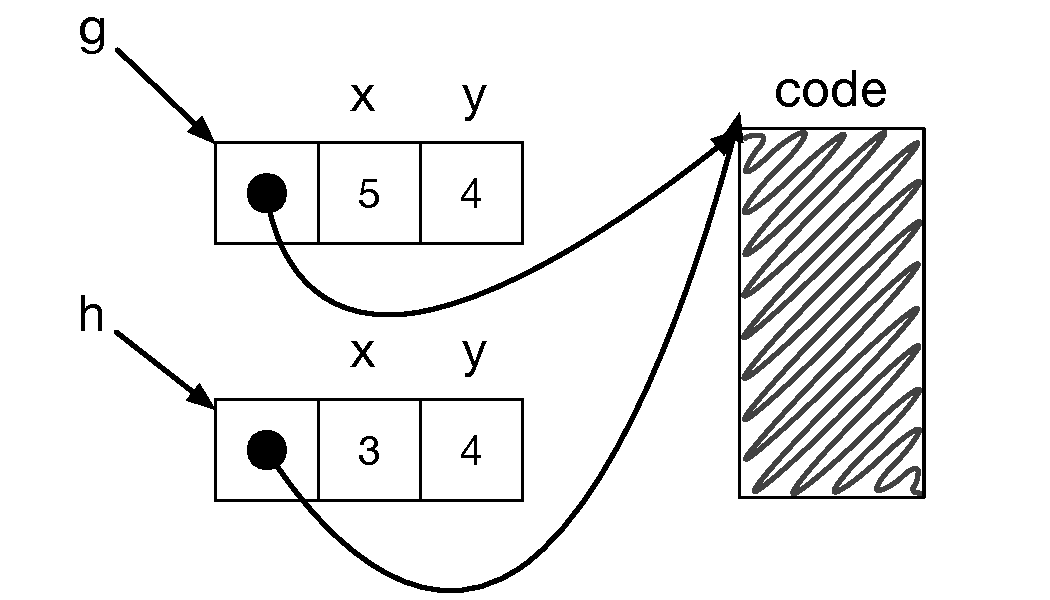
\includegraphics[width=0.6\textwidth]{figures/closures}
\caption{闭包示意图}
\label{fig:closure-eg}
\end{figure}

\begin{figure}[tbp]
  \begin{minipage}{0.8\textwidth}
% tests/lambda_test_6.rkt
\begin{lstlisting}[basicstyle=\ttfamily\footnotesize]
(define (f [x : Integer]) : (Integer -> Integer)
  (let ([y 4])
    (lambda: ([z : Integer]) : Integer
      (+ x (+ y z)))))

(define (main) : Integer
  (let ([g ((fun-ref f) 5)])
    (let ([h ((fun-ref f) 3)])
      (+ (g 11) (h 15)))))
\end{lstlisting}
$\Rightarrow$
\begin{lstlisting}[basicstyle=\ttfamily\footnotesize]
(define (f [clos2 : _] [x : Integer]) : (Vector ((Vector _) Integer -> Integer))
  (let ([y 4])
    (vector (list (fun-ref lambda2) x y))))

(define (lambda2 [clos3 : (Vector _ Integer Integer)] [z : Integer]) : Integer
  (let ([x (vector-ref clos3 1)])
    (let ([y (vector-ref clos3 2)])
      (+ x (+ y z)))))

(define (main) : Integer
  (let ([g (let ([clos5 (vector (list (fun-ref f6)))])
             ((vector-ref clos5 0) clos5 5))])
    (let ([h (let ([clos6 (vector (list (fun-ref f6)))])
               ((vector-ref clos6 0) clos6 3))])
      (+ ((vector-ref g 0) g 11) ((vector-ref h 0) h 15)))))
\end{lstlisting}
\end{minipage}

\caption{闭包转换示例}
\label{fig:colure-conversion-eg}
\end{figure}


\subsection{赋值对闭包的影响}

考虑下面这个例子:

\begin{lstlisting}
(define (f) : (-> Integer)
  (let ([x 0])
    (let ([g (lambda: () : Integer x)])
      (begin
        (set! x 42)
        g))))
((f))
\end{lstlisting}

函数 f 中定义了局部变量 x,初始值为0。
然后定义了一个无参匿名函数,函数体只有一个表达式 x。
也就是它什么都不做,直接返回 x。
接着我们把 x 的值改为 42,然后返回刚才的匿名函数。
我们期望\code{((f))}的返回值是 42。

但是上一小节描述的闭包转换会把正在编译闭包时x的值,也就是 0,放入闭包中。
这样编译出来的程序就会返回错误的结果 0。

并且,虽然x是函数f的局部变量,它的生命周期却超过了 f的生命周期。
这说明了自由变量的生命周期是不确定的。
在这个例子中,函数f执行结束后就退出了,但局部变量 x 仍然需要被匿名函数访问。
只有当这个匿名函数也无法被访问到时,我们才可以放心地清理掉变量 x。
因此,自由变量的值需要存放在堆上。
我们通常使用“box”来表示这种在堆上分配单个值的行为,“unbox”则指代对box的解引用。
这里我们并不需要引入 box 结构,单元素的向量就是box。

虽然理论上来说自由变量的生命周期是不确定的,但并非所有的自由变量我们都要放在堆上。
对于那些在代码中只有定义,没有重新被赋值的变量,
我们还是可以简单地把它们的值放在闭包中。
由于box会引入额外的开销,因此在本文的实现中,
只有那些可能被重新赋值的(也就是在代码中出现在\code{set!}语句中的)自由变量才会被box。
上面例子中的f函数,在转换后将得到以下结果。

\begin{lstlisting}
(define (f) : (-> Integer)
  (let ([x (vector 0)])
    (let ([g (lambda: () : Integer
               (vector-ref x 0))])
      (begin
        (vector-set! x 0 42)
        g))))
\end{lstlisting}


% !TeX root = ../../main.tex

\section{内存管理}

这一节讨论堆上的内存数据(在本文中只有向量这一种数据类型)以及如何管理堆内存。

堆内存与过程调用栈相互区分开,栈上的数据在函数退出后就无法再被访问了。
而堆允许我们通过引用来在不同的代码之间访问运行时创建的数据。
也正因此,堆上的数据的生命周期是不确定的。

\begin{lstlisting}
(let ([v (vector (vector 44))])
  (let ([x (let ([w (vector 42)])
             (let ([_ (vector-set! v 0 w)])
               0))])
    (+ x (vector-ref (vector-ref v 0) 0))))
\end{lstlisting}

例如在上面这个例子中,变量 w 的生命周期在绑定完 x 后就结束了,
但它指向的向量在这之后仍然可以被访问到,
因此上面这段代码的结果是0和42相加,也就是42。
我们在前一节讨论闭包时也使用了单元素向量来延长自由变量的生命周期。

从程序员可观察行为的角度来看,向量永远存在。
当然,如果它们真的永远存在,堆将越来越大,最终耗尽内存。
我们的语言必须实现自动地清理那些肯定不会再用到的数据,也就是垃圾回收。


\subsection{垃圾回收算法}

本文使用的是一个较为简单的垃圾回收算法:双空间拷贝回收\cite{Wilson_1992}。
图\ref{fig:copying-collector}给出了在垃圾回收之前(上面)和之后(下面)的内存情况。
在双空间收集器中,堆分为两个部分,分别命名为 FromSpace 和 ToSpace 。
最初,所有向量都分配到 FromSpace,当某次分配请求发现剩余的空间不够时,回收器开始工作。

\begin{figure}[t]
\centering
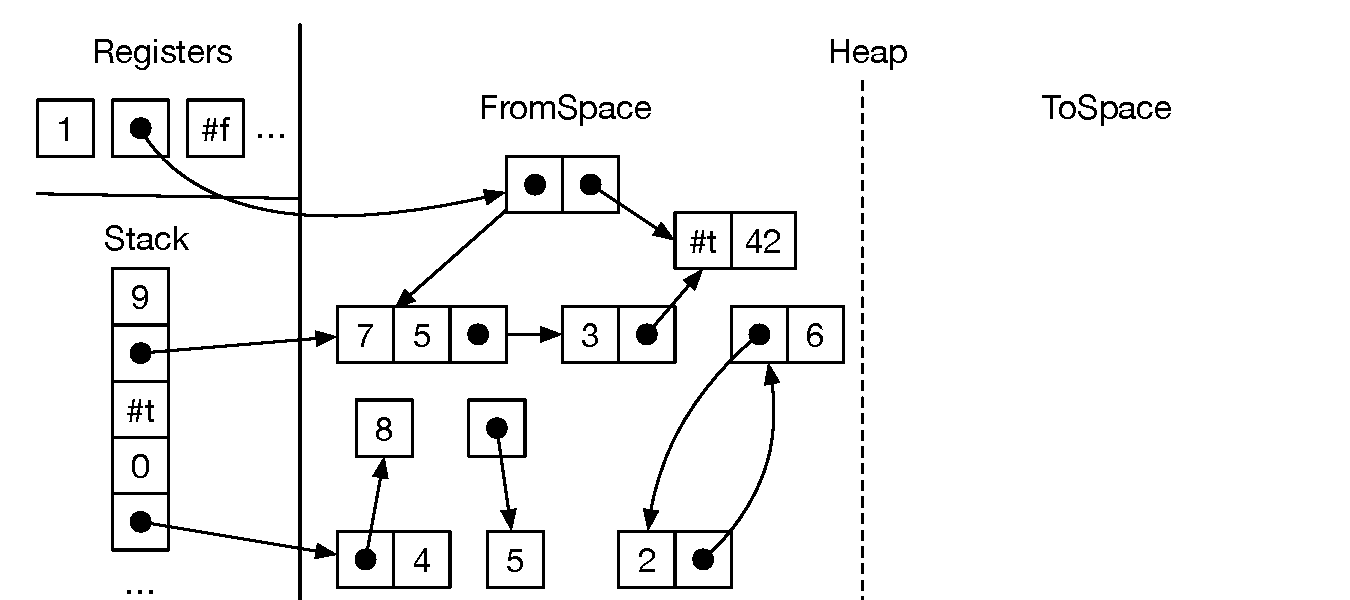
\includegraphics[width=\textwidth]{figures/copy-collect-1} \\[5ex]
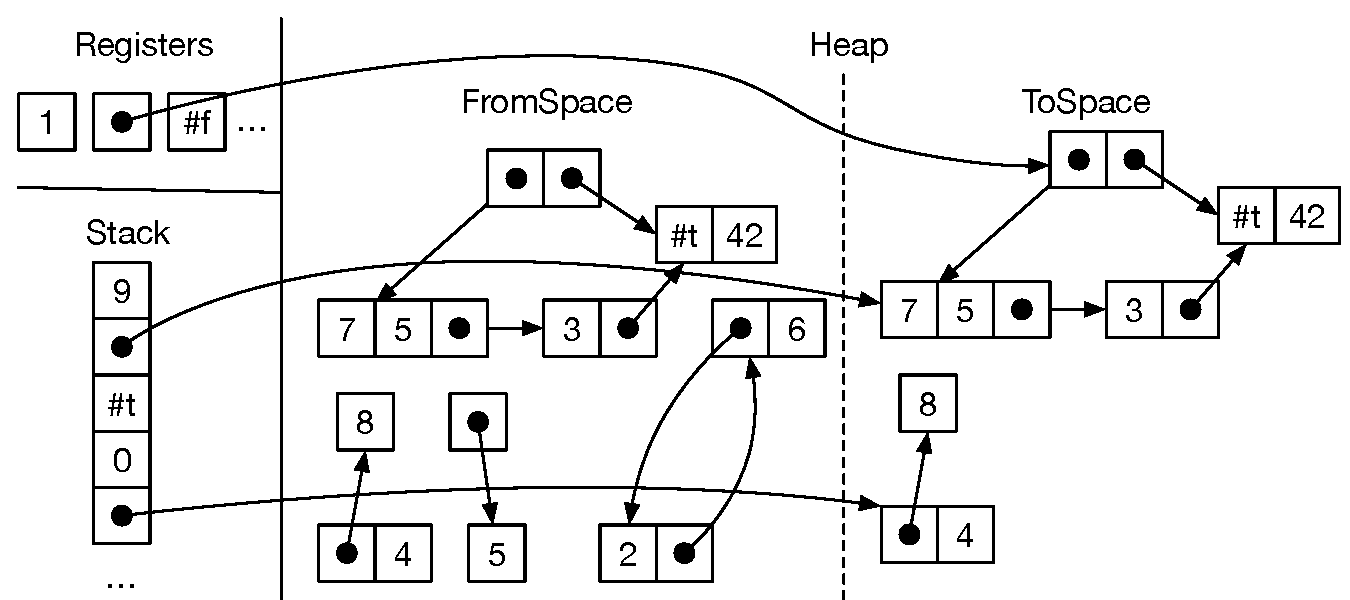
\includegraphics[width=\textwidth]{figures/copy-collect-2}
\caption{双空间拷贝回收示意图}
\label{fig:copying-collector}
\end{figure}

由于程序的行为是无法预知的,我们不可能准确地知道哪些向量在以后会被使用,哪些是垃圾。
但是我们可以保留下从当前所有变量出发,能访问到的那些向量,它们可能会被使用,也可能不会,
但剩余的不可达的向量一定是垃圾。

首先,地址存放在寄存器和栈上的向量自然是可达的,我们把它们称为根集。
从根集出发,所有能遍历到的向量均是活向量。
然后,我们把所有的活向量拷贝到ToSpace中,并把ToSpace当成新一轮的FromSpace,
在里面分配接下来的数据,原来的FromSpace则当成下一次的ToSpace。

在图\ref{fig:copying-collector}的例子中,根集中有三个指针,
一个在寄存器中,两个在堆栈中。所有活向量都以保留指针间的关系的方式复制到 ToSpace。
例如,寄存器中的指针仍然指向一个二元向量,
它的第一个元素是一个三元向量,第二个元素是一个二元向量。
有 4 个向量不能从根集到达,因此不需要复制到 ToSpace 中。

像这样的拷贝回收器的优点是分配数据很快(只需要看一下FromSpace的剩余空间是不是够),
没有碎片,可以回收包含循环引用的垃圾,回收的时间复杂度取决于有用的数据大小,而不是垃圾量。
主要缺点是它浪费了一半的内存,并且执行回收需要花长时间进行图遍历,
后者可以使用分代回收算法加以优化。


\subsection{拷贝回收}

我们仔细看一下活对象拷贝的过程。
堆上的对象和指针可以被视为一个图,我们需要复制那些从根集可以到达的结点。
图遍历算法如深度优先搜索或宽度优先搜索通过标记哪些顶点已经被避免重复遍历,
从而确保算法的终止。
这些遍历算法还需要使用栈或队列等数据结构。
本文使用宽度优先搜索和Cheney\cite{Cheney_1970}的链表紧凑算法中的一个技巧,
在拷贝数据到ToSpace的同时使用ToSpace来表示队列。

\begin{figure}[tbp]
\centering
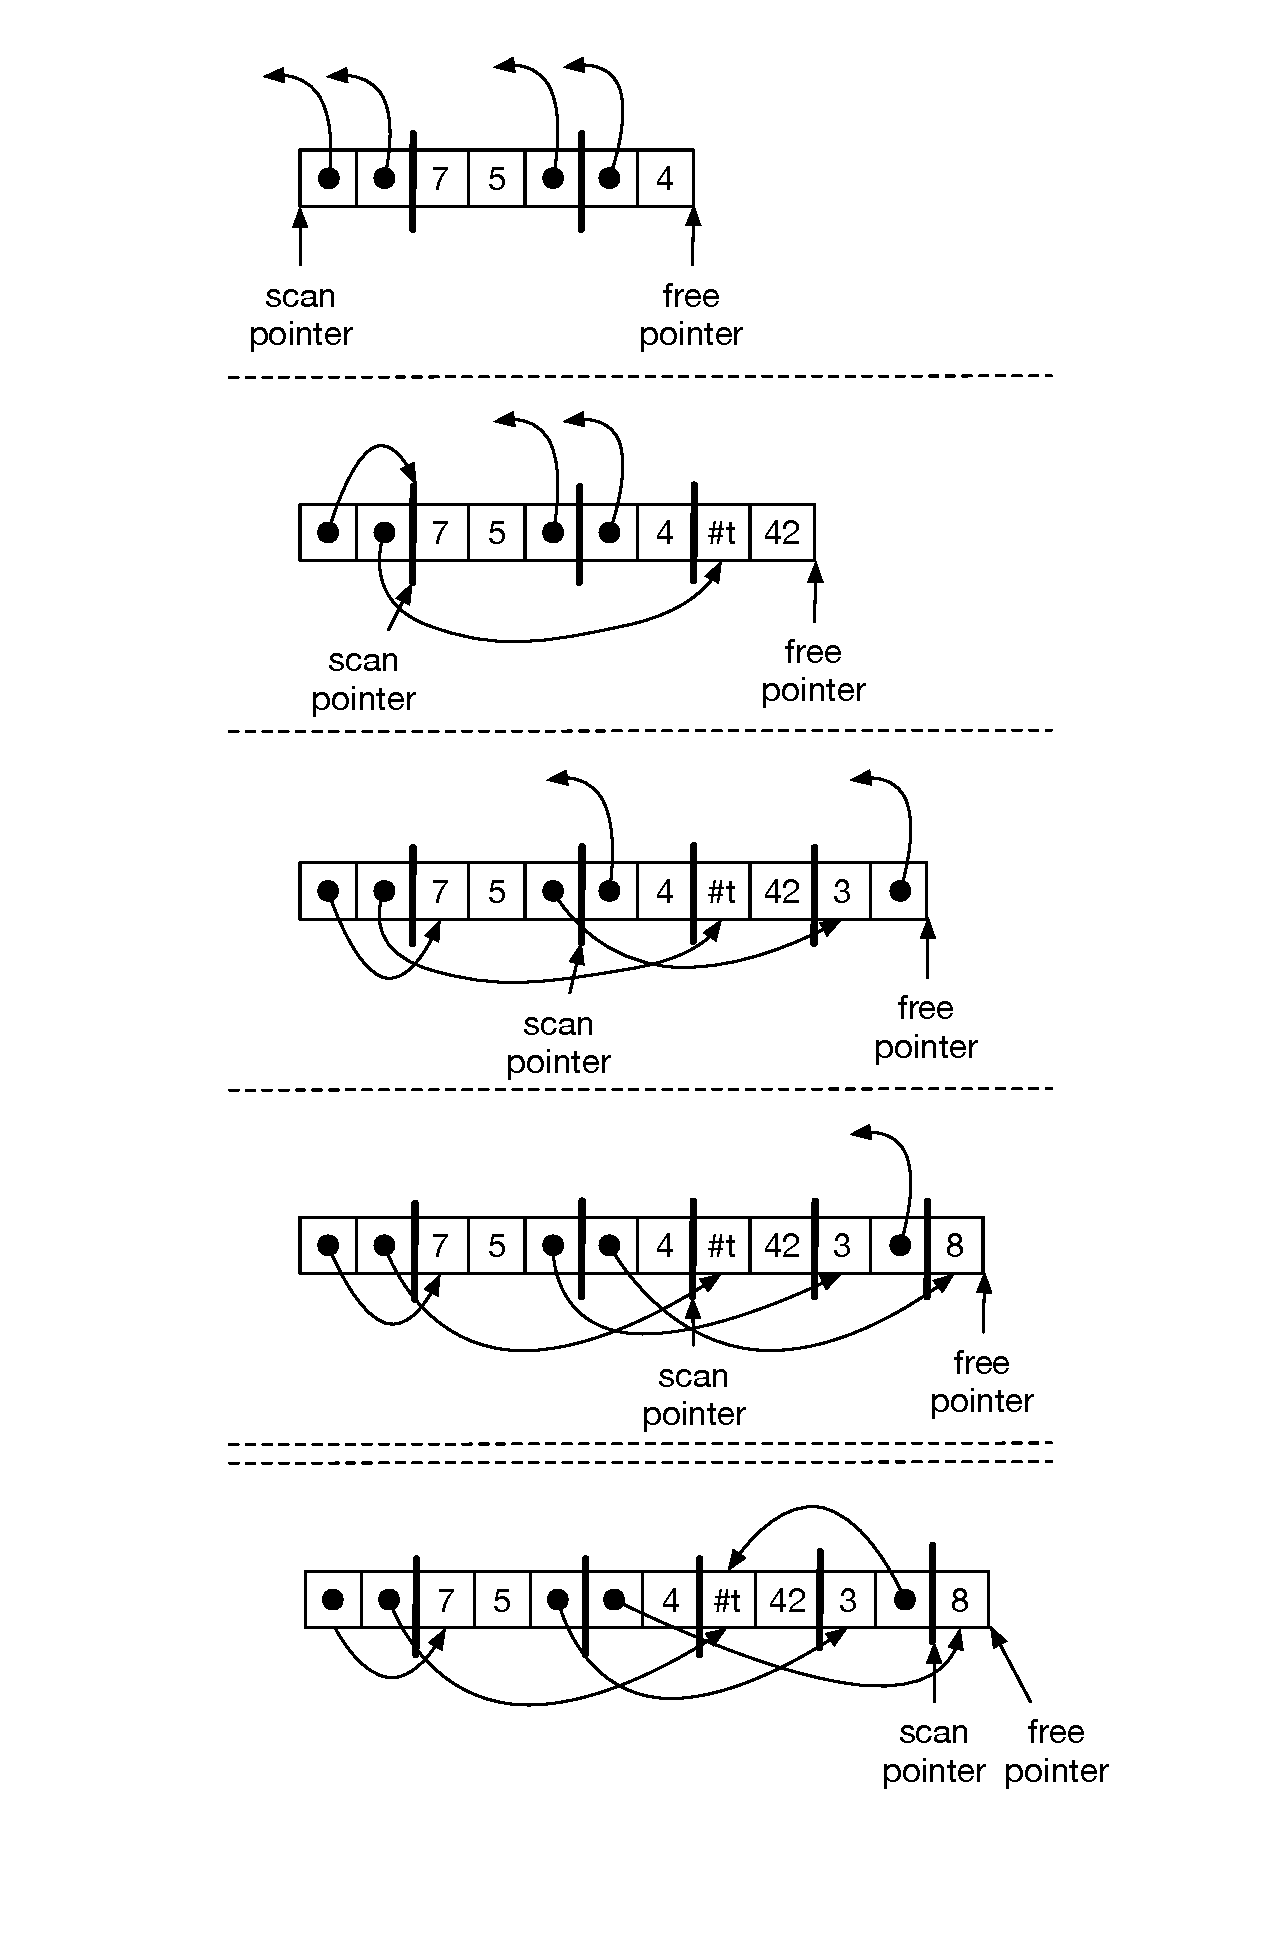
\includegraphics[width=0.9\textwidth]{figures/cheney}
\caption{拷贝回收的详细过程}
\label{fig:cheney}
\end{figure}

图\ref{fig:cheney}展示了在拷贝过程中 ToSpace 的几个瞬间。
队列由 ToSpace 开头的一块连续内存表示,使用两个指针跟踪队列的头和尾。
该算法首先将所有可以立即从根集到达的向量复制到 ToSpace 中,以形成初始队列。
当复制一个向量时,将旧向量标记为已被访问。下一小节将会讨论如何完成这个标记。
注意,队列中复制的向量内的任何指针仍然指向 FromSpace。
创建好初始队列后,算法将进入一个循环,
在循环中,算法会考察队头的向量,
将从该向量所有可以直接到达的向量复制到ToSpace并放到队尾(后移队尾指针),
然后更新队头向量中指针,使它们指向新复制的向量,
之后队头向量出队(后移队头指针),重复循环,直至队列为空,也就是队头指针赶上队尾指针。

在图\ref{fig:cheney}中,开始时队列中有三个向量。
队头向量的第一个元素指向的FromSpace中的一个被标记为已访问的向量,
这个已访问过的向量会保存它的克隆体在ToSpace中的地址(这一点在下一小节详细说明),
在这个例子中正是ToSpace中的第二个向量,因此我们把这个指针改为指向第二个向量。

队头向量的第二个元素是指向FromSpace中一个内容为\code{\#t}和\code{42}的向量,
并且它没有被标记为已访问。我们把它复制过来,放在队尾,并修改队头向量中的指针。
同时,我们还要标记FromSpace中的旧向量为已访问,
并在其中记录它的克隆体的地址(同样,见下一小节)。
此时队头向量处理完毕,我们后移队头指针,然后重复这个过程,直至队列为空。


\subsection{向量在内存中的表示}

首先,垃圾回收器需要区分指针和其他类型的数据。本文的实现策略如下:
对于指向根集的那些指针,我们不放在寄存器或者普通的过程调用栈上,
而是放在一个单独的栈上,这个栈当然也会随着函数的调用和返回相应地出栈入栈一些数据,
我们这个栈称作根栈,也叫影子栈。

而对于向量中的指针和非指针数据,我们通过在每个向量的开头增加一个额外的64位标签来实现。
图\ref{fig:tuple-rep}展示了两个示例,
注意这个图是以大端方式绘制的,从右到左,位置 0(最低位) 在最右边,
它对应着 x86 移动指令 salq (左移) 和 sarq (右移) 的方向。
“指针掩码”部分用于标记向量中哪些元素是指针,1代表为指针,0则为其他类型的数据。
指针掩码从第 7位开始,总共占 50位,因此该语言最多只允许长度为50的向量。
元组的长度 (元素的数量) 存储在位 1 到 6 的位置。
位置 0 则是我们的访问标记,如果它的值是1,则表示没有被访问,也就是还没有被复制到 ToSpace。
如果值是0,则说明这个向量已经被访问过了,
并且此时整个标签实际上是一个地址,表示的是复制后的向量在ToSpace中的位置。
(因为我们的所有数据都是64位的倍数,所以的向量8 字节对齐的,它们的地址的低 3 位总是 0。)

\begin{figure}[t]
\centering
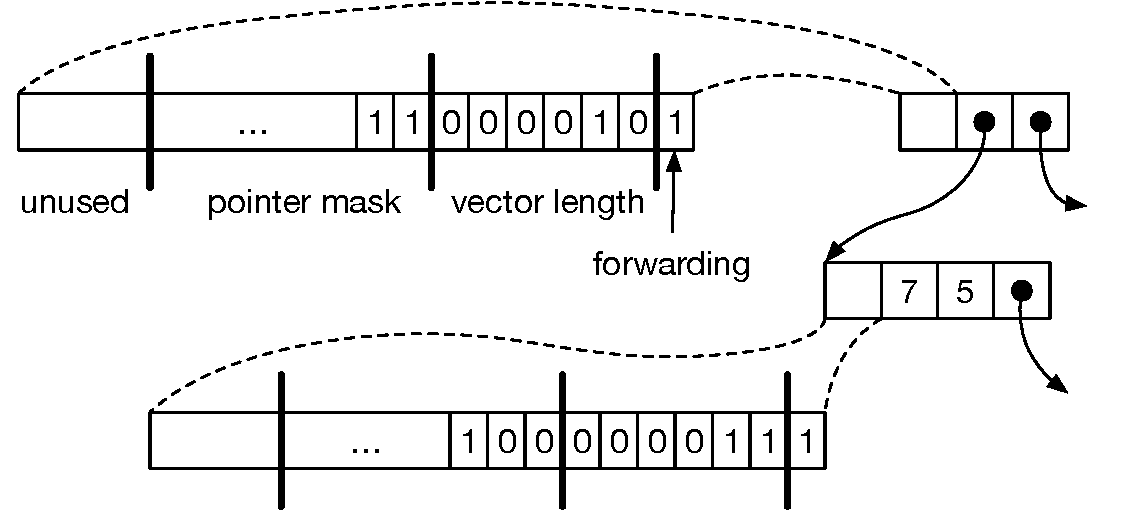
\includegraphics[width=0.8\textwidth]{figures/tuple-rep}
\caption{向量在内存中表示}
\label{fig:tuple-rep}
\end{figure}


\subsection{展开向量定义}

我们用c语言来实现垃圾回收器,编译生成一个目标文件,
和我们的编译器翻译出的汇编代码生成的目标文件一起链接成最终的可执行文件。
这个垃圾回收器提供了如下所示的几个接口。
\begin{lstlisting}
void initialize(uint64_t rootstack_size, uint64_t heap_size);
void collect(int64_t** rootstack_ptr, uint64_t bytes_requested);
int64_t* free_ptr;
int64_t* fromspace_begin;
int64_t* fromspace_end;
int64_t** rootstack_begin;
\end{lstlisting}

initialize 函数初始化 FromSpace、ToSpace 和根栈,在主函数的准备工作中被调用。
initialize 函数将 FromSpace 开头的地址放入全局变量 free\_ptr 中。
全局变量 fromspace\_end 指向的地址是 FromSpace 的最后一个元素的后面一个位置。
rootstack\_begin 变量指向根栈的第一个元素。

只要 FromSpace 中还有剩余空间,生成的代码就可以通过向前移动 free\_ptr 来分配向量。
FromSpace 中剩余的空间是 fromspace\_end 和 free\_ptr之间的差值。
当 FromSpace 中没有足够的空间留给下一次分配时,就调用 collect 函数。
collect 函数接受一个指向根栈当前顶部的指针 (栈顶元素的后面一个位置) 和需要分配的字节数。
collect 函数执行前文描述的复制回收过程。

编译器需要把一个简单的定义向量的语句翻译成一系列语句:
1) 把向量的各个元素的表达式绑定到一系列临时变量上;
2) 判断FromSpace是否有足够的空间,如果不够则调用 collect 函数;
3) 调用 allocate 函数;
4) 初始化向量。

\begin{lstlisting}
(vector |$e_0 \ldots e_{n-1}$|)
|$\Longrightarrow$|
(let ([|$x_0$| |$e_0$|]
      [|$x_{n-1}$| |$e_{n-1}$|]
      ...)
  (begin
    (if (< (+ (global-value free_ptr) |\itm{bytes}|)
           (global-value fromspace_end))
        (void)
        (collect |\itm{bytes}|))
    (let ([|$v$| (allocate |\itm{len}| |\itm{type}|)])
      (begin
        ([_ (vector-set! |$v$| |$0$| |$x_0$|)])
        ([_ (vector-set! |$v$| |$n-1$| |$x_{n-1}$|)])
        |$v$|))))
\end{lstlisting}

其中 allocate 接受参数len和向量的类型。
len指的是向量的长度,而 bytes 是需要为向量分配的总字节数,
即len加上1(一个64位的标签)再乘以8。
allocate 指令后续将被翻译为若干条汇编指令,包括根据向量的类型来计算标签的值。


% !TeX root = ../../main.tex

\section{原子化操作数}

前面已经提到过,汇编语言指令的操作数不允许放置复杂表达式,
只能是一个立即数或寄存器或内存位置。
我们通过为每一个复杂的操作数引入一个新的 let 绑定,
将复杂操作数绑定到新变量,然后使用新变量来代替复杂操作数,
就像下面这样。

\begin{transformation}
\begin{lstlisting}
(let ([x (+ 42 (- 10))])
  (+ x 10))
\end{lstlisting}
\compilesto
\begin{lstlisting}
(let ([x (let ([tmp1 (- 10)])
            (+ 42 tmp1))])
   (+ x 10))
\end{lstlisting}
\end{transformation}

本文使用两个相互递归的函数:\code{rco-atom} 和 \code{rco-exp} 来实现这个过程。
其思想是将 \code{rco-atom} 应用于需要成为原子的子表达式,
将 \code{rco-exp} 应用于不需要原子化的子表达式。

\code{rco-exp} 函数根据需要在其子表达式上分别调用
\code{rco-atom} 和 \code{rco-exp}。
\code{rco-atom}同样要对其接受的表达式分类讨论,
继续在复合子表达式上相应的调用\code{(+ 42 (- 10))}或\code{rco-exp}。
\code{rco-atom} 函数会返回两个东西:
一个原子化的表达式(一个变量或者一个数字之类的)
和一个将临时变量映射到原来的复杂操作数的列表。
\code{rco-exp} 根据这个列表创造出一系列的 let 绑定,
包裹在原表达式外面,并把原表达式的那些复杂操作数用原子化后的表达式进行替换。

在上面的例子中,对表达式\code{(+ 42 (- 10))}应用\code{rco-exp}函数,
\code{rco-exp}会对子表达式 \code{42} 和 \code{(- 10)} 分别应用\code{rco-atom}。
前者返回42和空列表,后者返回变量tmp1和把tmp1映射到表达式\code{(- 10)}的列表。

\begin{transformation}
\begin{lstlisting}
            (- 10)
\end{lstlisting}
\compilesto
\begin{lstlisting}
       tmp1
       ((tmp1 . (- 10)))
\end{lstlisting}
\end{transformation}

低效的实现可能会导致冗余变量的产生。
我们要确保\code{rco-exp}只对需要的原子化的子表达式调用\code{rco-atom},
\code{rco-atom}则要确保不要为本身就已经是原子的表达式再创建临时变量。



% !TeX root = ../../main.tex

\section{显示化控制流}
\label{sec:control}

这一趟编译过程将把我们的语言翻译成类似四元式的序列,
复杂的控制结构将会变成一些包含跳转语句的简单的语句序列。考虑下面的程序:

\begin{multilinecode}
\begin{lstlisting}
(let ([y (let ([x 20])
           (+ x (let ([x 22]) x)))])
  y)
\end{lstlisting}
\end{multilinecode}

前面描述的编译过程会把程序翻译成左边的结果,
显示化控制流则进一步得到右边的过程:
三
\begin{transformation}
\begin{lstlisting}
  (let ([y
      (let ([x1 20])
        (let ([x2 22])
          (+ x1 x2)))])
    y)
\end{lstlisting}
\compilesto
\begin{lstlisting}
    start:
      x1 = 20;
      x2 = 22;
      y = (+ x1 x2);
      return y;
\end{lstlisting}
\end{transformation}

我们先来考虑最简单的情况:假设程序不包含分支指令,
也不包含可变变量带来的结构,
即只关心最后一个表达式的返回值的\code{Begin}语句和循环语句。
那么程序就只剩下变量定义和运算
(当然还有函数,但是这趟编译过程正是针对每个函数单独处理的,
而函数调用则和运算按同样的方式处理)。
可以看到,就像上面的例子一样,最终的结果就是一系列的赋值语句和一个返回语句。
返回语句是由处于尾位置的表达式编译得到的为。尾位置的定义如下:

(1) \code{(FunctionDef params body)}中,\code{body}处于尾位置。

(2) 如果 \code{(let x e body)} 处于尾位置,则\code{body}处于尾位置。


我们使用两个相互递归的函数explicate-tail 和 explicate-assign 来实现,如图\ref{fig:explicate-control-implementation}所示。

\begin{figure}[t]
\begin{center}
\vspace{0.4em}
\begin{tabular}{c}
\begin{lstlisting}
(define (explicate-tail e)
  (match e
    [(or (Int n))
     (Return (Int n))]
    [(Let x rhs body)
     (let ([instructions (explicate-tail body)])
       (explicate-assign rhs x instructions))]
    ...
    ))

(define (explicate-assign e x cont)
  (match e
    [(Int n)
     (append (Assign (Var x) (Int n))
             cont)]
    [(Let y rhs body)
     (let ([new-cont (explicate-assign body x cont)])
       (explicate-assign rhs y new-cont))]
    ...))
\end{lstlisting}
\end{tabular}
\vspace{0.8em}
\end{center}

    \caption{显示化控制流的实现}
    \label{fig:explicate-control-implementation}
\end{figure}
\begin{multilinecode}
\end{multilinecode}

explicate-tail 函数应用于位于尾位置的表达式,
而 explicate-assign 函数应用于出现在 \key{let} 右侧的表达式。
二者都返回一串四元式。

如果\code{explicate-tail}收到的表达式不是\code{let}表达式,
那么就简单的返回一个四元式\code{return}。
如果是let,那么let中的body部分就属于尾位置,
对其递归调用\code{explicate-tail},得到一串四元式instructions,
把变量名,let语句的右侧,以及这串四元式作为参数传递给\code{explicate-tail}。
\code{explicate-tail}对let语句的右侧表达式进行判断,
如果不是let,那么生成一个赋值四元式,把这个右侧表达式赋给变量名,然后添加到那串四元式的前面即可。
这里用参数名cont来接收四元式序列,意思正是这串四元式将会变成赋值语句的continue。
而如果let的右侧又是一个let,
我们则应当先调用\code{explicate-tail}把这个内部let的body赋给外面的变量,
得到一个新的cont,把它和内部let的变量名和右侧表达式再一次传给\code{explicate-tail}。
就像上面的例子,我们先把\code{(+ x1 x2);}赋给y,\code{return y;}作为其cont,
然后再把这两条语句作为为\code{x1, x2}赋值的语句的cont。
可以说,这一趟编译过程生成四元式序列的过程是倒过来的。
这种实现方式被叫做累积传递风格。

接下来我们考虑上分支语句和赋值,扩展尾位置的定义。
\begin{enumerate}
\item 如果 \code{(if pred then else)} 处于尾位置,
  则表达式\code{then}和\code{else}均处于尾位置。
\item 如果 \code{(begin ... final-e)}处于尾位置,则 \code{final-e}处于尾位置。
\end{enumerate}

与此类似,我们再定义谓词位置和副作用位置,
并相应地定义\code{explicate-pred}和\code{explicate-effect}函数。
\code{explicate-effect}接收cont,
\code{explicate-pred}则接收then-cont和else-cont,
它们也都返回一串四元式序列。
加入分支后,\code{explicate-pred}函数中要生成一些跳转语句,
分别指向then-cont和else-cont。
最终,这趟编译过程将能够完成下面这样的转换:

\begin{transformation}
\begin{lstlisting}
(let ([x (read)])
  (let ([y (read)])
    (if (if (< x 1)
            (eq? x 0)
            (eq? x 2))
        (+ y 2)
        (+ y 10))))
\end{lstlisting}
\compilesto
\begin{lstlisting}
start:
   x = (read);
   y = (read);
   if (< x 1) goto block40;
   else goto block41;
block40:
   if (eq? x 0) goto block38;
   else goto block39;
block41:
   if (eq? x 2) goto block38;
   else goto block39;
block38:
   return (+ y 2);
block39:
   return (+ y 10);
\end{lstlisting}
\end{transformation}


% !TeX root = ../../main.tex

\section{生成汇编}
\label{sec:x86}

这一步我们会将上一节中生成的四元式序列转换为x86汇编指令序列。
把四元式转换成汇编指令的过程非常直白,
因为四元式只有运算、赋值、函数调用、跳转等少数几种可能的类别,
并且运算的操作数和函数调用的参数都是原子表达式。
唯一的难点在于四元式包含变量,变量名当然是无穷多的,
但x86没有变量,他只有寄存器和过程调用栈。
在生成汇编这趟过程中,我们保留这些变量名,
在下一趟编译过程再把这些变量放到合适的寄存器或栈上去。

接下来我们举一些典型的四元式来说明生成汇编的过程。
首先是整数运算操作,以加法为例:
\begin{transformation}
\begin{lstlisting}
    |$\itm{var}$| = (+ |$\Atm_1$| |$\Atm_2$|);
\end{lstlisting}
\compilesto
\begin{lstlisting}
    movq |$\Arg_1$|, |$\itm{var}$|
    addq |$\Arg_2$|, |$\itm{var}$|
\end{lstlisting}
\end{transformation}

翻译运算操作时要注意可以优化的情况。
比如,如果加法的一个参数与赋值的左边的变量相同,那么就不需要额外的 move 指令。
整个赋值语句可以被翻译成一条 addq 指令:
\begin{transformation}
\begin{lstlisting}
    |$\itm{var}$| = (+ |$\Atm_1$| |$\itm{var}$|);
\end{lstlisting}
\compilesto
\begin{lstlisting}
    addq |$\Arg_1$|, |$\itm{var}$|
\end{lstlisting}
\end{transformation}

read 函数在 x86 汇编中没有直接对应的功能,
所以我们在 runtime.c 中用 C 语言实现一个 \code{read\_int} 函数来提供这个功能。
前文提到,runtime.c 中还包括垃圾回收器以及一些全局变量,
这些功能合在一起被称为“运行时系统”,或简称为“运行时”。
\begin{transformation}
\begin{lstlisting}
    |$\itm{var}$| = (read);
\end{lstlisting}
\compilesto
\begin{lstlisting}
    callq read_int
    movq %rax, |$\itm{var}$|
\end{lstlisting}
\end{transformation}

Return语句的翻译方法和上面两个例子是一样的,只要把赋值左边的var改为\%rax即可。
对于布尔值真和假,我们把它们分别编译成立即数1和0。
然后是布尔运算\code{not}:
\begin{transformation}
\begin{lstlisting}
    |$\itm{var}$| = (not |$\Atm$|);
\end{lstlisting}
\compilesto
\begin{lstlisting}
    movq |$\Arg$|, |$\itm{var}$|
    xorq $1, |$\itm{var}$|
\end{lstlisting}
\end{transformation}
和整数运算一样,这里也需要考察atm来判断能否优化进而减少一条指令。
接下来我们看一下x86对布尔运算和条件分支提供的支持。

cmpq 指令比较它的两个参数来确定一个参数是小于、等于还是大于另一个参数。
cmpq 指令在参数的顺序和结果放置的位置上不太一样。
参数顺序是颠倒的:如果我们想知道 x 是不是小于 y,就需要写 \code{cmpq y, x}。
cmpq 的结果被放置在特殊的 EFLAGS 寄存器中。
这个寄存器不能直接访问,但可以通过许多指令进行查询。
指令 \code{set}cc \code{d} 根据条件代码 cc
(e 表示等于,l 表示小于,le 表示不等于,g 表示大于,ge 表示大于等于),
将立即数 1 或 0 放入目标 d 中。
还需要注意的是d必须是单字节寄存器,例如al或 ah,它们是 rax 寄存器的一部分。
movzbq 指令可以将单个字节寄存器中的值移到 64 位寄存器里。
综上所述,\code{eq?}运算可以被这样翻译:
\begin{transformation}
\begin{lstlisting}
    |$\itm{var}$| = (eq? |$\Atm_1$| |$\Atm_2$|);
\end{lstlisting}
\compilesto
\begin{lstlisting}
    cmpq |$\Arg_2$|, |$\Arg_1$|
    sete %al
    movzbq %al, |$\Var$|
\end{lstlisting}
\end{transformation}

再来看 if 表达式的编译。
指令 \code{j}cc label 更新程序计数器指向 label 之后的指令,
这取决于 EFLAGS 寄存器中的结果是否与条件代码 cc 匹配,
否则条件跳转指令还是继续执行下一条指令。
因为条件跳转指令依赖于 EFLAGS 寄存器,
所以通常它前面会立即有一个 cmpq 指令来设置 EFLAGS 寄存器。

\begin{transformation}
\begin{lstlisting}
if (eq? |$\Atm_1$| |$\Atm_2$|) goto |$\ell_1$|;
else goto |$\ell_2$|;
\end{lstlisting}
\compilesto
\begin{lstlisting}
    cmpq |$\Arg_2$|, |$\Arg_1$|
    je |$\ell_1$|
    jmp |$\ell_2$|
\end{lstlisting}
\end{transformation}

接下来考虑和向量有关的指令。我们保留r11寄存器,专门用它来访问向量也就是堆上的数据。
\begin{transformation}
\begin{lstlisting}
|$\itm{var}$| = (vector-ref |$\itm{vec}$| |$n$|);
\end{lstlisting}
\compilesto
\begin{lstlisting}
movq |$\itm{vec}$|, %r11
movq |$8(n+1)$|(%r11), |$\itm{var}$|
\end{lstlisting}
\end{transformation}

\begin{transformation}
\begin{lstlisting}
(vector-set! |$\itm{vec}$| |$n$| |$\itm{arg}$|);
\end{lstlisting}
\compilesto
\begin{lstlisting}
movq |$\itm{vec}$|, %r11
movq |$\itm{arg}$|, |$8(n+1)$|(%r11)
\end{lstlisting}
\end{transformation}

\begin{transformation}
\begin{lstlisting}
|$\itm{vec}$| = (allocate |$n$| |$\itm{type}$|);
\end{lstlisting}
\compilesto
\begin{lstlisting}
movq free_ptr(%rip), %r11
addq |$8(n+1),$| free_ptr(%rip)
movq $|$\itm{tag}$|, 0(%r11)
movq %r11, |$\itm{var}$|
\end{lstlisting}
\end{transformation}

\begin{transformation}
\begin{lstlisting}
    (collect |$\itm{bytes}$|);
\end{lstlisting}
\compilesto
\begin{lstlisting}
movq %r15, %rdi
movq $|\itm{bytes}|, %rsi
callq collect
\end{lstlisting}
\end{transformation}

\code{free\_ptr}中的地址是FromSpace中的下一个空闲地址,把它赋给\code{r11},
然后把它向前移动$8(n+1)$ 个字节以留出足够的空间来放置向量的内容
(每个元素是8个字节(64位),以及一个64位的标签)。
在编译时我们通过type信息计算出标签,放到向量的第0号位置。
标签的组成参见图~\ref{fig:tuple-rep}处的描述。
对垃圾回收函数collect的调用被编译成对运行时里的collect函数的调用,
参数分别是根栈的顶部地址和需要分配的字节数。
我们还保留了r15寄存器,专门用来保存指向根栈顶部的指针,它会在主程序的准备工作中被初始化。

最后是函数。对于每个函数定义,我们都需要把参数从参数寄存器里移到对应的变量名中:
\begin{transformation}
\begin{lstlisting}
       start:
          |$\itm{instr}_1$|
          |$\vdots$|
          |$\itm{instr}_n$|
\end{lstlisting}
\compilesto
\begin{lstlisting}
    start:
       movq %rdi, |$x_1$|
       movq %rsi, |$x_2$|
       |$\vdots$|
       |$\itm{instr}_1$|
       |$\vdots$|
       |$\itm{instr}_n$|
\end{lstlisting}
\end{transformation}

函数赋值给变量成为 load-effective-address 指令:
\begin{transformation}
\begin{lstlisting}
    |$\itm{var}$| = (fun-ref |$f$|);
\end{lstlisting}
\compilesto
\begin{lstlisting}
    leaq (fun-ref |$f$|), |$\itm{var}$|
\end{lstlisting}
\end{transformation}

然后是函数调用,正如第\ref{sec:call-in-x86}节中所述,它们被编译成x86的间接函数调用:
\begin{transformation}
\begin{lstlisting}
|\itm{var}| = (call |\itm{fun}| |$\itm{arg}_1~\itm{arg}_2\ldots$|));
\end{lstlisting}
\compilesto
\begin{lstlisting}
    movq |$\itm{arg}_1$|, %rdi
    movq |$\itm{arg}_2$|, %rsi
    |$\vdots$|
    callq *|\itm{fun}|
    movq %rax, |\itm{var}|
\end{lstlisting}
\end{transformation}

如果函数调用是尾巴调用,如第\ref{sec:tail-call}节所述,
我们要把上面的callq换成jmp,并在其前面加上弹出当前栈帧的一系列指令,
但由于此时我们还没有进行寄存器分配,也没有生成函数的结束工作,
我们不知道这些指令具体都有哪些,因此我们在这里引入一个临时的\code{TailJmp}指令来替换callq,
后续分配完寄存器之后再把它替换成完整的弹出栈帧和跳转指令。



% !TeX root = ../../main.tex

\section{寄存器分配}

这一步将会把前一节生成的包含变量的x86指令变成真正的x86指令,
包含三个步骤:活变量分析、建立变量之间的干涉图、根据干涉图分配寄存器或内存。

\subsection{活变量分析}

在程序中的某一个点,如果一个变量或寄存器的当前包含的内容在后面会被使用,
我们就说这个变量或寄存器在当前这个点是活的。

我们需要计算出每条指令后所有活变量的集合,
对于不包含分支指令的简单情况,我们从后往前计算按下面的方法计算。

设$I_1,\ldots, I_n$ 为指令序列。
记指令 $I_k$ 之后的活变量集为$L_{\mathsf{after}}(k)$ ,
 $I_k$ 之前为活变量集为 $L_{\mathsf{before}}(k)$ 。
一条指令之后的活变量集与下一条指令之前的活变量集相同。
\begin{equation} \label{eq:live-after-before-next}
L_{\mathsf{after}}(k) = L_{\mathsf{before}}(k+1)
\end{equation}
开始时,在最后一条指令之后没有活变量,所以
\begin{equation}\label{eq:live-last-empty}
L_{\mathsf{after}}(n) = \emptyset
\end{equation}
然后我们重复应用以下规则,将指令序列从后向前遍历。
\begin{equation}\label{eq:live-before-after-minus-writes-plus-reads}
L_{\mathsf{before}}(k) = (L_{\mathsf{after}}(k) - W(k)) \cup R(k)
\end{equation}
其中 $W(k)$ 是指令 $I_k$ 中写入数据的变量或寄存器,
$R(k)$ 是指令 $I_k$ 中读取数据的变量或寄存器。

注意callq 指令应该在其写集 $W$ 中包含所有调用者保存寄存器,
因为这些寄存器可能在函数调用期间被被调用者使用。
同样,callq 指令应当根据调用的函数的参数个数,
在其读集 $R$ 中包含适当的参数传递寄存器。

从显示化控制流这一编译过程的输出开始,编译器的中间形式就从原来的树变成了图。
每个标签下的一系列四元式或者一系列汇编指令,
一直到下一个标签或者到结束,被称作一个基本块。
跳转指令可以从一个基本块跳转到另一个基本块。
二者分别作为有向图的顶点和边,构成了控制流图(CFG)\cite{Allen_1970}。

加入了分支和循环之后,我们要考虑两个问题。第一个问题是跳转指令的活变量分析。
假设第k条指令是跳转指令,它指向某一个基本块,
记该基本块的第一条指令前面的活变量集为$L_{\mathsf{before'}}(1)$。
如果是无条件跳转指令,则
\begin{equation}\label{eq:live-jmp}
L_{\mathsf{before}}(k) = L_{\mathsf{before'}}(1)
\end{equation}
如果是条件跳转指令,则
\begin{equation}\label{eq:live-jmpcc}
L_{\mathsf{before}}(k) = L_{\mathsf{before'}}(1) \cup L_{\mathsf{before}}(k+1)
\end{equation}

第二个问题是以什么样的顺序、重复多少次才能计算出各个基本块中各指令的$L_{\mathsf{after}}$。
解决方法如下:对控制流图进行拓扑排序,选择最末尾的一个基本块开始分析,
计算块内指令的live-after以及块的live-before,也就是第1条指令的live-before,
如果块的live-before中的活变量在这趟分析后增加了,
那么对于所有能跳转这个基本块的块都再进行一次分析,
重复进行下去,直到所有块的live-before集合都不再增大。
这种迭代分析控制流图的方法叫作数据流分析\cite{Kildall_1973},
它也适用于许多其他静态分析问题。
\begin{comment}
下面的代码描述了这一迭代过程。其中\code{trans-G}是转置后的控制流图,
用以计算哪些基本块指向了某一个块,
\code{label->live}是一个字典,用于记录每个基本块的live-before集合。

\begin{lstlisting}
(while (not (queue-empty? worklist))
  (define label (dequeue! worklist))
  (define-values (new-block new-live-before)
    (uncover-live-block (dict-ref blocks label) label->live))
  (hash-set! new-blocks label new-block)
  (unless (equal? new-live-before (hash-ref label->live label))
    (hash-set! label->live label new-live-before)
    (for ([label^ (in-neighbors trans-G label)])
      (enqueue! worklist label^))))
\end{lstlisting}
\end{comment}


\subsection{使用图着色算法进行分配}

知道了任意时刻的活变量集合,我们就能知道某两个变量能不能被分配到同一个寄存器:
如果它们在某一时刻同时是活变量,那我们显然不能把它们分配到同一个寄存器。
把这种情况称之为两个变量互相干涉。我们创建一个无向图,称之为干涉图,
顶点是所有变量,然后在所有干涉的变量之间添加边。

接下来就是为图上的变量分配寄存器,
用从 0 到k − 1 的整数对应于可以用来分配变量的 k 个寄存器。
整数 k 及以上对应的是堆栈位置。
这样一来寄存器分配就变成了图着色问题,这些整数就是可以使用的颜色,
有边的顶点之间不能分配相同的颜色。

本文使用的图着色算法是DSATUR算法\cite{Brélaz_1979}。
其中 SATUR 是饱和度的缩写,它指的是一个顶点上的约束。
我们为某一个顶点涂上一个颜色后,
所有与它相邻的顶点就不能再选用这个颜色,也就多了一个约束。
DSATUR算法每次都选择一个约束最多的顶点,给他涂上编号尽可能小的颜色,
然后给相邻的为上色顶点加上约束,再在剩下的未上色顶点中重复这个过程。

图着色完成后,我们就为所有变量都分配了一个寄存器或者一个栈上的空间。
x86代码已经大致生成完毕,接下来只需要再整理一下一些不合法的x86指令,
再添加上函数的准备工作和结束工作指令即可。


% !TeX root = ../main.tex

\section{整理指令}

我们生成的x86指令中还存在一些不符合规范的地方。
比如,x86中一条指令最多访存一次,
而前面的编译过程可能会生成包含两次内存引用的代码,
这时我们可以利用保留的rax寄存器做一次中转:

\begin{transformation}
\begin{lstlisting}
movq -8(%rbp), -16(%rbp)
\end{lstlisting}
\compilesto
\begin{lstlisting}
  movq -8(%rbp), %rax
  movq %rax, -16(%rbp)
\end{lstlisting}
\end{transformation}

如果间接函数调用指令的操作数没有被分配到寄存器上,
而是使用了栈空间,我们同样要做一次中转:
\begin{transformation}
\begin{lstlisting}
     callq *-8(%rbp)
\end{lstlisting}
\compilesto
\begin{lstlisting}
  movq -8(%rbp), %rax
  callq *%rax
\end{lstlisting}
\end{transformation}

前面的编译过程会引入很多临时变量,
而图着色算法会把一些变量分配到同一个寄存器或栈位置,
这就可能出现一些movq指令,它的两个操作数是一样的,我们可以直接把这些指令删除掉。

最后就是为每个函数生成第\ref{sec:call-in-x86}节中描述的准备工作和结束工作。
在准备工作中,我们要把所有用到的被调用方保留寄存器存入栈中,
因为这里面可能存放着调用这个函数的调用方的一些数据。
结束工作中再把这些内容逆序弹出回这些寄存器里。
准备工作中还要根据程序中向量的数量移动根栈指针r15。
相应地,在结束工作中也需要把它移动回去。

生成了结束工作后,我们还要把\ref{sec:x86}一节中临时创造的\code{TailJmp}指令换成
真正的间接跳转指令\code{jmp *\%rax},
并在它的前面插入结束工作中除了retq之外的指令。
最后,主程序的准备工作者还需要初始化垃圾回收器,
即调用垃圾回收器的\code{initialize}函数和
把根栈顶部\code{rootstack\_begin}送入根栈指针寄存器r15。

至此,所有的编译工作均已完成,编译器已经能够将一段源程序编译成正确、合法的x86汇编程序,
并且能和runtime.o一起被GCC编译套件链接生成一个能在x86-64平台的Linux系统上运行的可执行文件。


\section{本章小结}

本章详细描述了从源程序中解析出抽象语法树后到生成可执行文件的所有编译过程,
其中每一节对应了对中间表示,也就是语法树或四元式的一趟或若干趟转换,
包括其作用和目的以及具体的算法或转换示例。本章也是本文工作的重点。
